\documentclass[12pt]{article}
\usepackage[utf8]{inputenc}
\usepackage[T1]{fontenc}
\usepackage{titlesec}
\usepackage[inline]{enumitem}
\usepackage[left=2.54cm,top=3cm,right=2.54cm,bottom=3cm]{geometry}
\PassOptionsToPackage{hyphens}{url}\usepackage{hyperref}
\usepackage[format=hang, labelfont=it, textfont=it]{caption}

\usepackage[sorting=none, style=numeric-comp]{biblatex}

\usepackage{pdfpages}
\usepackage{float}
\usepackage{graphicx}
\usepackage{tabularx}
\usepackage{setspace}
\usepackage{framed}
\usepackage{listings}
\usepackage{epigraph}
% To have two column glossary
\usepackage[acronym,toc,nogroupskip,nopostdot]{glossaries}
\usepackage{glossary-mcols}
% % \usepackage[table]{xcolor}
%\usepackage[acronym,toc]{glossaries}

\renewcommand{\arraystretch}{1.15}


\graphicspath{ {00images/} }
\DeclareGraphicsExtensions{.png,.PNG,.pdf}
% \DeclareGraphicsExtensions{.pdf,.png,.PNG} % - CHANGE TO THIS

\addbibresource{references.bib}
\setlength{\parindent}{1cm}

% Acronyms %%%%%%%%
\makeglossaries
% TODO check abbreviation capitalisation consistency

\newacronym{xacml}{XACML}{eXtensible Access Control Markup Language}
\newacronym{pdp}{PDP}{Policy Decision Point}
\newacronym{saml}{SAML}{Security Assertion Markup Language}
\newacronym{idp}{IdP}{Identity Provider}
\newacronym{rp}{RP}{Relying Party}
\newacronym{nist}{NIST}{National Institute of Standards and Technology}
\newacronym{pii}{PII}{Personally Identifiable Information}
\newacronym{ial}{IAL}{Identity Assurance Level}
\newacronym{csp}{CSP}{Credential Service Provider}
\newacronym{aal}{AAL}{Authenticator Assurance Level}
\newacronym{fal}{FAL}{Federation Assurance Level}
\newacronym{fido}{FIDO}{Fast Identity Online}
\newacronym{ctap}{CTAP}{Client to Authenticator Protocol}
\newacronym{u2f}{U2F}{Universal Second Factor}
\newacronym{nfc}{NFC}{Near Field Communication}
\newacronym{ble}{BLE}{Bluetooth Low Energy}
\newacronym{usb}{USB}{Universal Serial Bug}
\newacronym{w3c}{W3C}{World Wide Web Consortium}
\newacronym{uaf}{UAF}{Universal Authentication Framework}
\newacronym{oidc}{OIDC}{OpenID Connect}
\newacronym{ms}{MS}{Microsoft}
\newacronym{op}{OP}{OpenID Connect Provider}
\newacronym{jwt}{JWT}{JSON Web Token}
\newacronym{url}{URL}{Uniform Resource Locator}
\newacronym{json}{JSON}{JavaScript Object Notation}
\newacronym{api}{API}{Application Programming Interface}
\newacronym{saas}{SaaS}{Software as a Service}
\newacronym{crm}{CRM}{Customer relationship management}
\newacronym{pacs}{PACS}{Physical access control system}
\newacronym{acs}{ACS}{Access control system}
\newacronym{sso}{SSO}{Single sign-on}
\newacronym{mfa}{MFA}{Multi-factor Authentication}
\newacronym{oath}{OATH}{Initiative for Open Authentication}
\newacronym{otp}{OTP}{One-time password}
\newacronym{ams}{AMS}{Access Management System}
\newacronym{esb}{ESB}{Enterprise Service Bus}
% \newacronym{}{}{}
% \newacronym{}{}{}
% \newacronym{}{}{}
% \newacronym{}{}{}
% \newacronym{}{}{}
% \newacronym{}{}{}

% TODO check abbreviation capitalisation consistency
\makeglossaries
%%%%%%%%%%%%%%%%%%% 

\begin{document}

% \includepdf{cover_page}
% \includepdf{page_zero}
\tableofcontents

\begin{singlespacing}

% To have two column glossary
\setglossarystyle{mcolindex}
% \setglossarystyle{long}
\printglossary[type=\acronymtype, title=List of acronyms and abbreviations, toctitle=List of acronyms and abbreviations, nonumberlist]
\printglossary
\end{singlespacing}

\section{Introduction}
% 
\acrfull{acs} are playing a crucial role in every enterprise. They are being used/implemented for both, the physical access to company premises, online and internal resources. There are countless of different systems and providers offering such systems, ranging from simple card access systems and password log-ins to complex ones combining different types of physical and online access to resources. 

The problem of today’s access systems is that they are usually handling physical and online accesses separately, two systems have to be implemented and companies are usually specializing in providing one of those systems. Companies such as HID\footnote{\url{https://www.hidglobal.com/solutions/access-control-systems}, accessed 26 March 2019} or G4S\footnote{\url{https://www.g4s.com/en-gb/what-we-do/security-services/fire-and-security-systems/symmetry-software}, accessed 26 March 2019} are providing physical \acrshort{acs} to enterprises which allows employees to access the building, rooms, canteen or garage based on their access levels. On the other hand, there are tech companies such as Microsoft\footnote{\url{https://docs.microsoft.com/en-us/windows-server/identity/ad-ds/get-started/virtual-dc/active-directory-domain-services-overview}, accessed 26 March 2019} which offer software for managing employees’ access to online services and resources.

% TODO Add reference!
Therefore, there exist two mostly independent systems intended for similar use cases. These systems are either managed individually or can be interconnected, so that there is one endpoint for managing accesses. Both approaches work fine, but what if there was an \acrshort{acs} which would combine both physical and online access? What if physical access would be possible by authenticating the employee with smartcard, smartphone or authenticator key? Simply, there would be a need only for one device, with which an employee would be able to access premises as well as authenticate himself when login-in to a service. Such a system not only solves the problem of the employees’ experience and convenience of having to carry around an access card, but also a problem of security of corporate account because of passwords. The reason is that many companies has policy that requires changes of password a few times a year and therefore, employees tend to use easy to remember passwords  as well as many corporate accounts has been “hacked” by phishing attacks\cite{} Canadian Business Banking Customers Hit With Targeted Phishing, Account Takeover Attacks REF!. This can be avoided by using physical authenticators instead of passwords.

The aim of this project is to address this problem and propose a system, where physical access control and online access control is managed from the single endpoint as it can be seen in Figure~\ref{fig:IntroArchitecture}. Another very important feature introduced by this system, is the possibility of using \acrshort{fido}2 \acrshort{nfc} enabled authenticator or smartphone to access a building, rooms or printers. Both devices would work similarly to an access card which is usually given to an employee. A device needs to be swiped in front of the reader or connected to a reader wirelessly, using \acrshort{ble} in case of smartphone, which allows or deny access. It is common these days, that employees get to use many online services with their corporate account. To avoid passwords, technology called \acrshort{fido}2 aims to get rid of passwords when logging into account by using an authenticator, either a physical key device or smartphone. This allows “strong authentication” (REF! Why Strong Authentication is a Critical Requirement for Improving Critical Infrastructure Cybersecurity). The only thing the employee needs to type in when logging-in is the user ID and then he needs a \acrshort{fido}2 authenticator which authenticates him, at least in our system. Because of that, the employee has no longer to carry an access card with him, and only needs smartphone or authenticator when accessing physical premises of enterprise, as well as it empowers him to “forget” about passwords when logging-in into online services by using the same smartphone and authenticator.

Secondary aim of this system lies in the access management, which grants or denies the entry or use of a service for an employee. 
%To facilitate this, policies, attributes or role-based access can be implemented, which enables assigning to each employee a role/s and  attributes or creating policies by which the access will be granted or denied automatically.

\begin{figure}[ht]
    \centering
    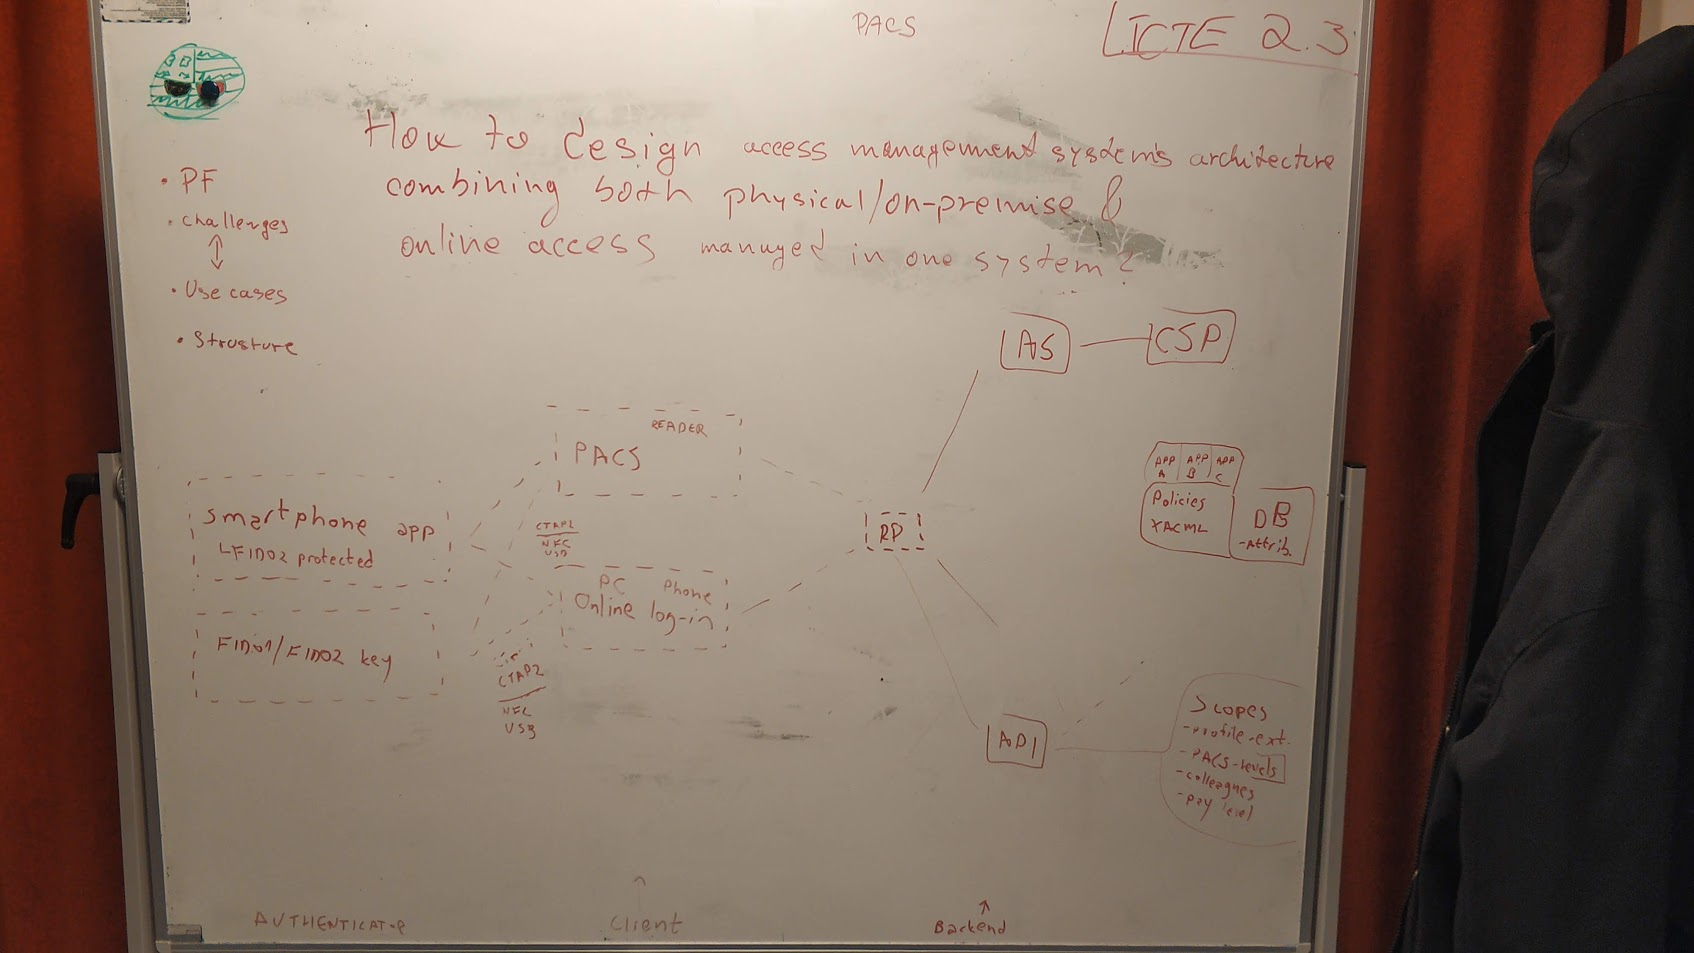
\includegraphics[width=.95\textwidth]{00images/IntroArchitecture}
    \caption{Explanation! + new diagram}
    \label{fig:IntroArchitecture}
\end{figure}

\subsection{Challenges} \label{challenges}

There is a number of challenges, which the current \acrshort{acs} in enterprises are facing. One of the major concerns of every access system is its security. Passwords are often targeted as the weakest link in the system. Every employee has their corporate account linked with many services and is accessing many protected resources. Often employees are forced to change their passwords periodically. Therefore, choosing a weak password and successful phishing attacks are a threat which can be solved by two-factor authentication, but as showed in \acrshort{nist} Special Publication 800-63B \cite{Grassi2017DigitalManagement} there are threats still associated with \acrshort{mfa} such as Social engineering, Phishing attacks or Endpoint compromise. Choosing a right combination of factors for authentication is therefore crucial.

Living in the era of fast technical advance, employees also require convenience when using access systems and carrying around an access card is not the most convenient method anymore, as shown in study by HID~\cite{2017AccessGlobal}, where 61\% of respondents sees integration between systems as hugely beneficial for user convenience or by Netflix~\cite{2012NetflixPilot}, where 87.5\% of respondents would like to use smartphones to open doors in the workplace for authentication. \acrshort{acs} should therefore, offer more convenient ways of authentication -- for example a smartphone.

Often, the physical access control and access policy management systems are two separate entities in enterprises. This requires more resources spend on managing these systems, as well as more set-up work when a new employee is hired or leaves the company. Having one system to handle these tasks is thus desirable.
\subsection{Problem formulation} \label{problemFormulation}
The motivation for this project comes from the existing split of online and physical access control systems. Secondary, the low security of passwords has been demonstrated by several phishing cases and their use is discouraged.
% TODO add reference here
Alternative ways of strong authentication have been proposed instead, including physical cryptographic devices.
% TODO add reference here
The banking industry, which has been using similar tokens for a long period of time already (credit cards), has now witnessed the migration of these tokens to smartphones, mainly for user convenience.
% TODO add reference here
Such migration is also technically possible in access control scenarios, although its use has been limited in practice.

Taking into account the challenges and issues mentioned previously, we propose an innovative \acrshort{acs} that addresses these issues, by building on top of state-of-the-art technologies in the field. The problem formulation is as follows:

\begin{center}
    \textit{“How to design an Access control system, combining both physical and online access control, that includes strong authentication and enables the use of smartphone?”}
\end{center}

\paragraph{Sub-questions}
We define the following sub-problems to help guide us in the analysis and design of the system:

% TODO Is this still draft?
\begin{itemize}[noitemsep]
    \item What solutions are there on the market?
    \item What is the system architecture?
    \item Which technologies are the best for proposed system?
    \item Which components of the system must be implemented for MVP?
    \item What are the requirements of the system?
\end{itemize}
\subsection{Report Structure}


\pagebreak
\section{Background}

% TODO section intro

\subsection{Basic terms}

\paragraph{Policy}
The IT portfolio of many current enterprises consists of a variety of different applications and systems. As a fine grained control of users' access to these resources is required, management of access rights for every user can become tedious. A set of rules is usually in place, which specify how a \textit{subject} (a person, user, actor) can interact with an \textit{object} (system, program), describing subject's accountability and capabilities within the object~\cite{Feltus2008PreliminaryConcept}. Policies are often used in the \hyperref[sec:xacml]{XACML} context.

\paragraph{Assertion}
An assertion is a ``confident and forceful statement of fact or belief''\footnotemark. In the context of authentication and in particular \hyperref[sec:saml]{SAML}, it is often the case that the identity provider is an independent entity, logically and physically separated from the application/relying party that requested user authentication. After the identity provider authenticates the user, it issues an assertion, confirming that the user's identity has been verified.

\footnotetext{\url{https://en.oxforddictionaries.com/definition/assertion}, accessed 05 March 2019}

\subsection{XACML}

 \acrfull{xacml} is a standardised, XML-based language for expressing security policies. It provides methods to define and combine security policies and to rapidly identify, which policy applies to a given subject. \acrshort{xacml} was first standardised by OASIS\footnote{\url{https://www.oasis-open.org/}, accessed 04 March 2019} in 2003 and the latest version is XACML 3.0, standardised in 2013~\cite{OASISStandard2013EXtensible3.0}. The further description is based on this latest version.
 
 The context of \acrshort{xacml} is illustrated in Figure~\ref{fig:xacml-context}. At the centre of the system is the \acrfull{pdp} which evaluates an input (such as access requests) against a policy set and issues an output -- a decision (such as \textit{access granted}). \acrshort{xacml} defines the formal language of the policy set and of the requests/responses. A policy set contains comprises one or more \textit{policies} and a \textit{policy combining algorithm}. The main components of a policy are a \textit{target} to which this policy applies and one or more \textit{rules}. The rule must specify a \textit{target} to which it applies and an \textit{evaluation} (\textit{permit} or \textit{deny}). It can also optionally specify \textit{conditions}, \textit{obligations} and \textit{advices}, all of which further shape the scope of the rule. Policy combining algorithm specifies the order and other conditions that decide, which policy will be finally applied on the request~\cite{OASISStandard2013EXtensible3.0}.
 
 \begin{figure}[ht]
    \centering
    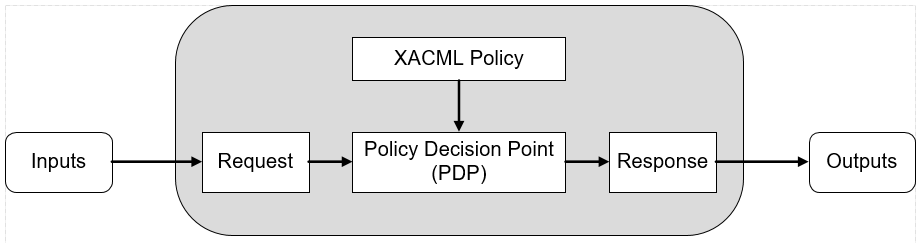
\includegraphics[width=.95\textwidth]{xacml-context}
    \caption{The context diagram of \acrshort{xacml}. From~\cite{OASISStandard2013EXtensible3.0}, edited.
    }
    \label{fig:xacml-context}
\end{figure}
 
The \acrshort{xacml} standard defines in detail several logical entities and their interactions. The native format for messages between these entities is XML, but a profile has been developed to support JSON message format~\cite{2017JSON1.0}. Additional profile was also created to describe implementation in a RESTful architecture~\cite{2017REST1.0}.
 
 Several implementations of \acrshort{xacml} exist in Java, Python and other languages. Criticisms of \acrshort{xacml} include low adoption rate, unsuitability for federated enterprises~\cite{Cser2013XACMLDead}, and lack of transparency for the end user~\cite{Cser2013XACMLDead, Ardagna2011ExpressiveApplications}.


\subsection{SAML}\label{sec:saml}

The \acrfull{saml} is a framework for exchange of assertions containing security information between two online parties, typically an identity provider and a relying party. Similarly as XACML, \acrshort{saml} was developed by OASIS. Version 1.0 was released in 2002 and version 2.0 (latest) in 2005. The rest of this report refers to version 2.0.

The main premise of \acrshort{saml} is that the \acrfull{idp} and the protected resource/application are two separated entities. This is desired, since it enables us to manage identities centrally for multiple applications and avoids duplication user accounts across these applications. Moreover, separating these enables both parts to specialise only in their task.

The Figure~\ref{fig:saml-architectire} illustrates the separation of these two entities. It also depicts the high-level flow of the authentication process. If the user wants to access the protected resource on the right, they first need to authenticate themselves with the \acrshort{idp}.

Another noteworthy aspect of \acrshort{saml} is the identity federation. This is achieved, when the \acrshort{idp} and the \acrshort{rp} are in different security realms, possibly operated by different organisations. As long as an agreement is established between the two, users can use identity managed by the \acrshort{idp} to access any resources outside the organisation's boundary~\cite{2008SecurityOverview}.

 \begin{figure}[ht]
    \centering
    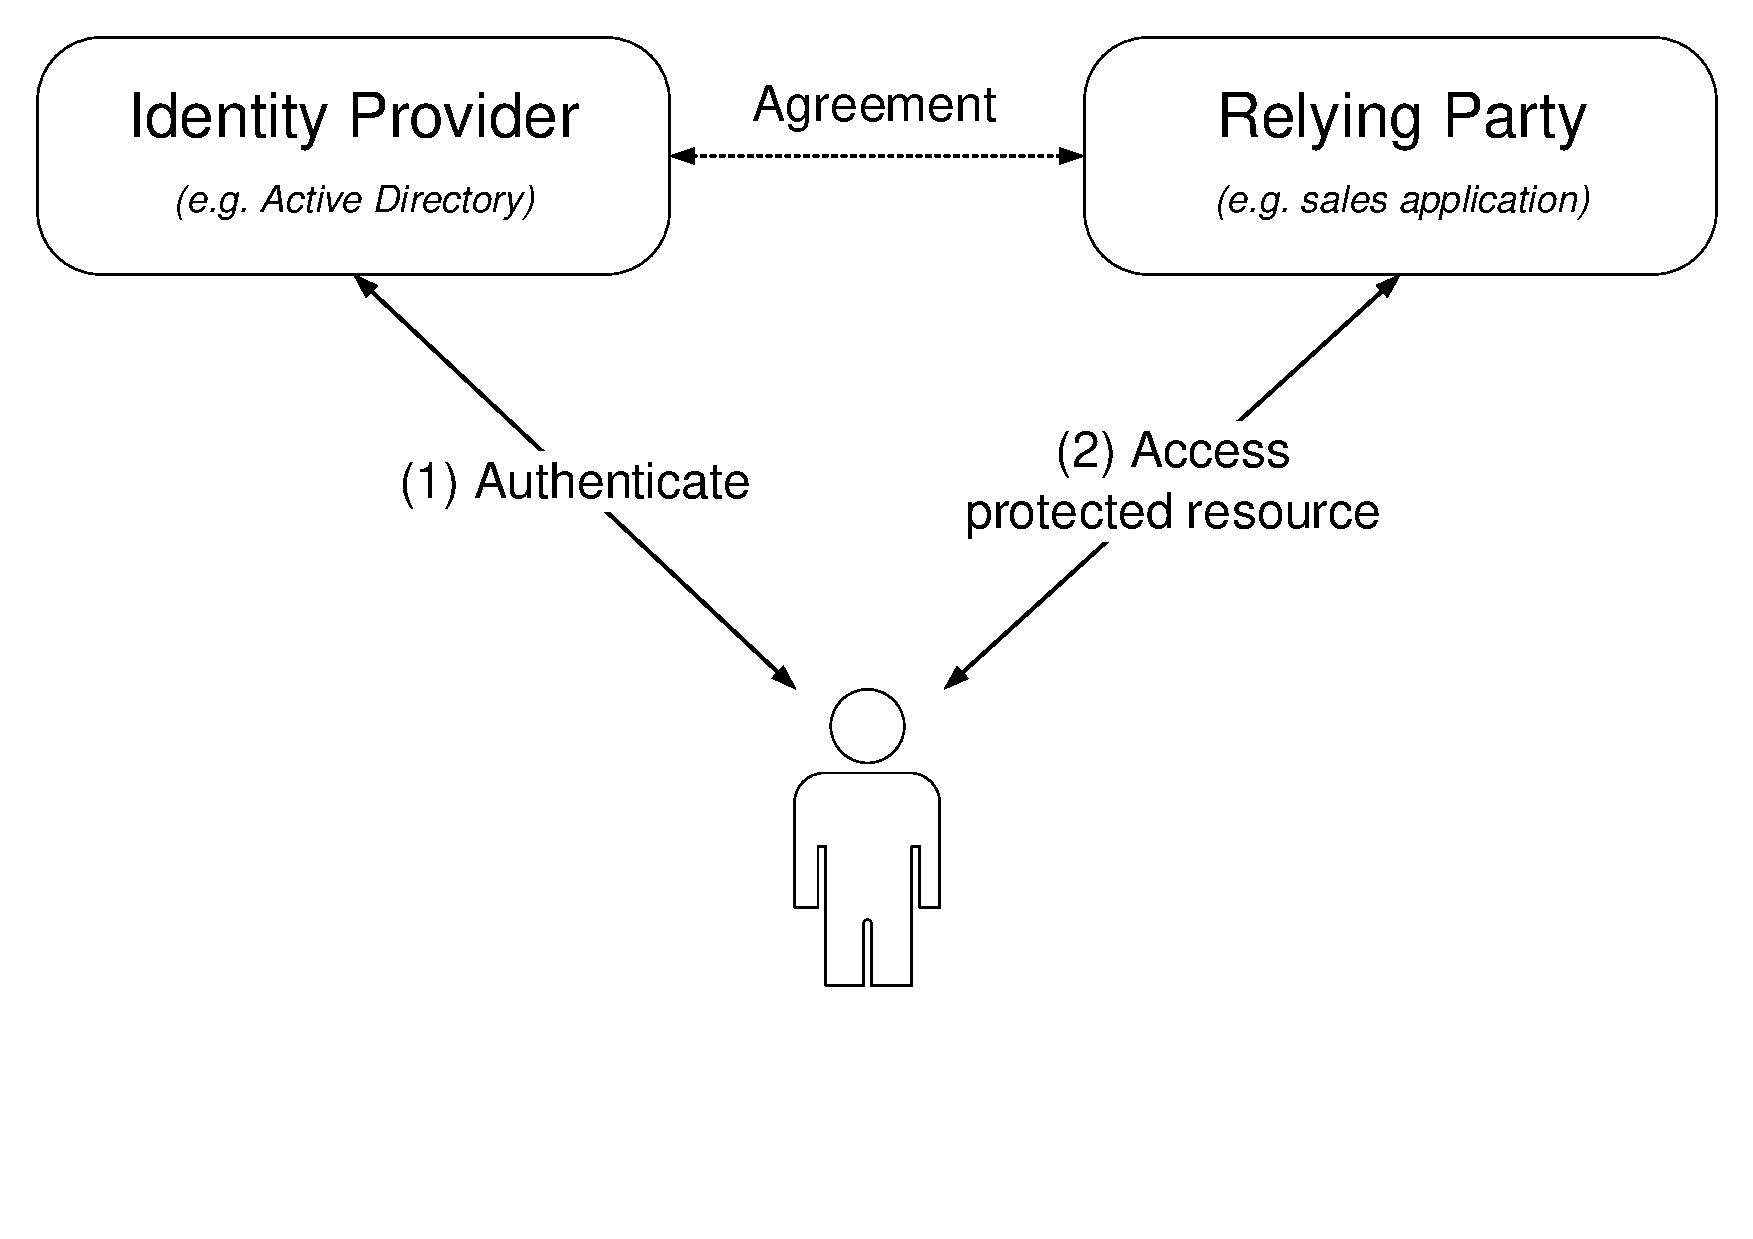
\includegraphics[width=.95\textwidth]{saml-architecture}
    \caption{The general use case of SAML, demonstrating the premise of functional separation of \acrshort{idp} and \acrshort{rp}. Taken from~\cite{2008SecurityOverview}.}
    \label{fig:saml-architectire}
\end{figure}

\paragraph{Assertions}
An assertion in \acrshort{saml} contains some security information about the \textit{subject}. Subject could be the user Bob and the associated information could be Bob's email address and job title. The security information need to be of one of following three categories:

\begin{enumerate*}[label=(\roman*)]
    \item \textit{Authentication statements} describe means and the timestamp of the authorisation carried out by the asserting party;
    \item \textit{Attribute statements} provide information about the subject; and
    \item \textit{Authorisation decision statement} describes what the subject is permitted to access in the system.
\end{enumerate*}

% \paragraph{Protocols}
% \acrshort{saml} defines a number of general protocols to facilitate the message exchange during different parts of the assertion process.

\paragraph{Bindings}
\acrshort{saml} describes how the messages exchanged during an assertion process can be bound to lower-level transport protocols. There are in total 6 bindings defined by the standard, but the following three are of particular interest:

\begin{itemize}[noitemsep]
    \item \textit{HTTP Redirect Binding}, where the entire \acrshort{saml} message is carried in the URL parameters, in the header of an HTTP GET method. This is suitable for short messages as the length of URL is limited in practice. This binding can be used in a RESTful system.
    \item \textit{HTTP POST Binding}, where the \acrshort{saml} message is base64 encoded into an XHTML form and transmitted using the HTTP POST method. This binding can also be used in a RESTful system.
    \item \textit{SAML SOAP Binding} specifies how the \acrshort{saml} messages are carried in an XML envelope over SOAP over any underlying transport protocol~\cite{Cantor2005BindingsV2.0}.
\end{itemize}

% \paragraph{Profiles}
% Several profiles which build on assertions and bindings are defined in the standard which correspond to the most common use cases of \acrshort{saml}. 

While \acrshort{saml} is widely adopted in the industry and is considered generally secure, numerous security flaws have been identified over time. Most of these arised from improper implementation of the protocol and have been patched since discovery~\cite{Krawczyk2014SecureAttacks}. The vulnerabilities included XML signature wrapping, assertion eavesdropping~\cite{Chen2014Environment-BoundAssertions} and XML parsing issues~\cite{Degges2018AVulnerability}.
\subsection{NIST Digital Identity Guidelines}

The \acrfull{nist} developed a set of guidelines, intended primarily to govern how public authorities in the US implement digital authentication in non-national-security scenarios. Yet, it was adopted by by wider community, spanning out of the government sector.
% REFERENCE Government Adopts an Industry Approach to Open Source Collaboration

The guidelines contain three volumes, covering three distinct areas of authentication:
\begin{enumerate*}[label=(\roman*)]
    \item SP 800-63A focused on Enrolment and Identity Proofing;
    \item SP 800-63B centred around Authentication and Lifecycle Management; and
    \item SP 800-63C covering federation and assertions.
\end{enumerate*}
The guidelines advertise the use of authentication to mitigate risks of unauthorised access to protected resources, but also promote minimising the collection of \acrfull{pii} and use of pseudonymous information whenever possible.
%REFERENCE Digital identity guidelines: revision 3

The guidelines define a Digital Identity Model (Figure~\ref{fig:nist-model}), which is useful to distinguish the various types of roles and activities within an authentication system. On the left side of the model there is a \acrfull{csp}. \acrshort{csp} is an entity that issues electronic credentials and registers user's \textit{authenticator} (authenticator is something that the user has or controls). On the right side of the model is the verifier, whose task is to authenticate users by validating binding of their authenticators to their credentials.
% %REFERENCE Digital identity guidelines: revision 3

 \begin{figure}[ht]
    \centering
    % TODO Change figure in visio
    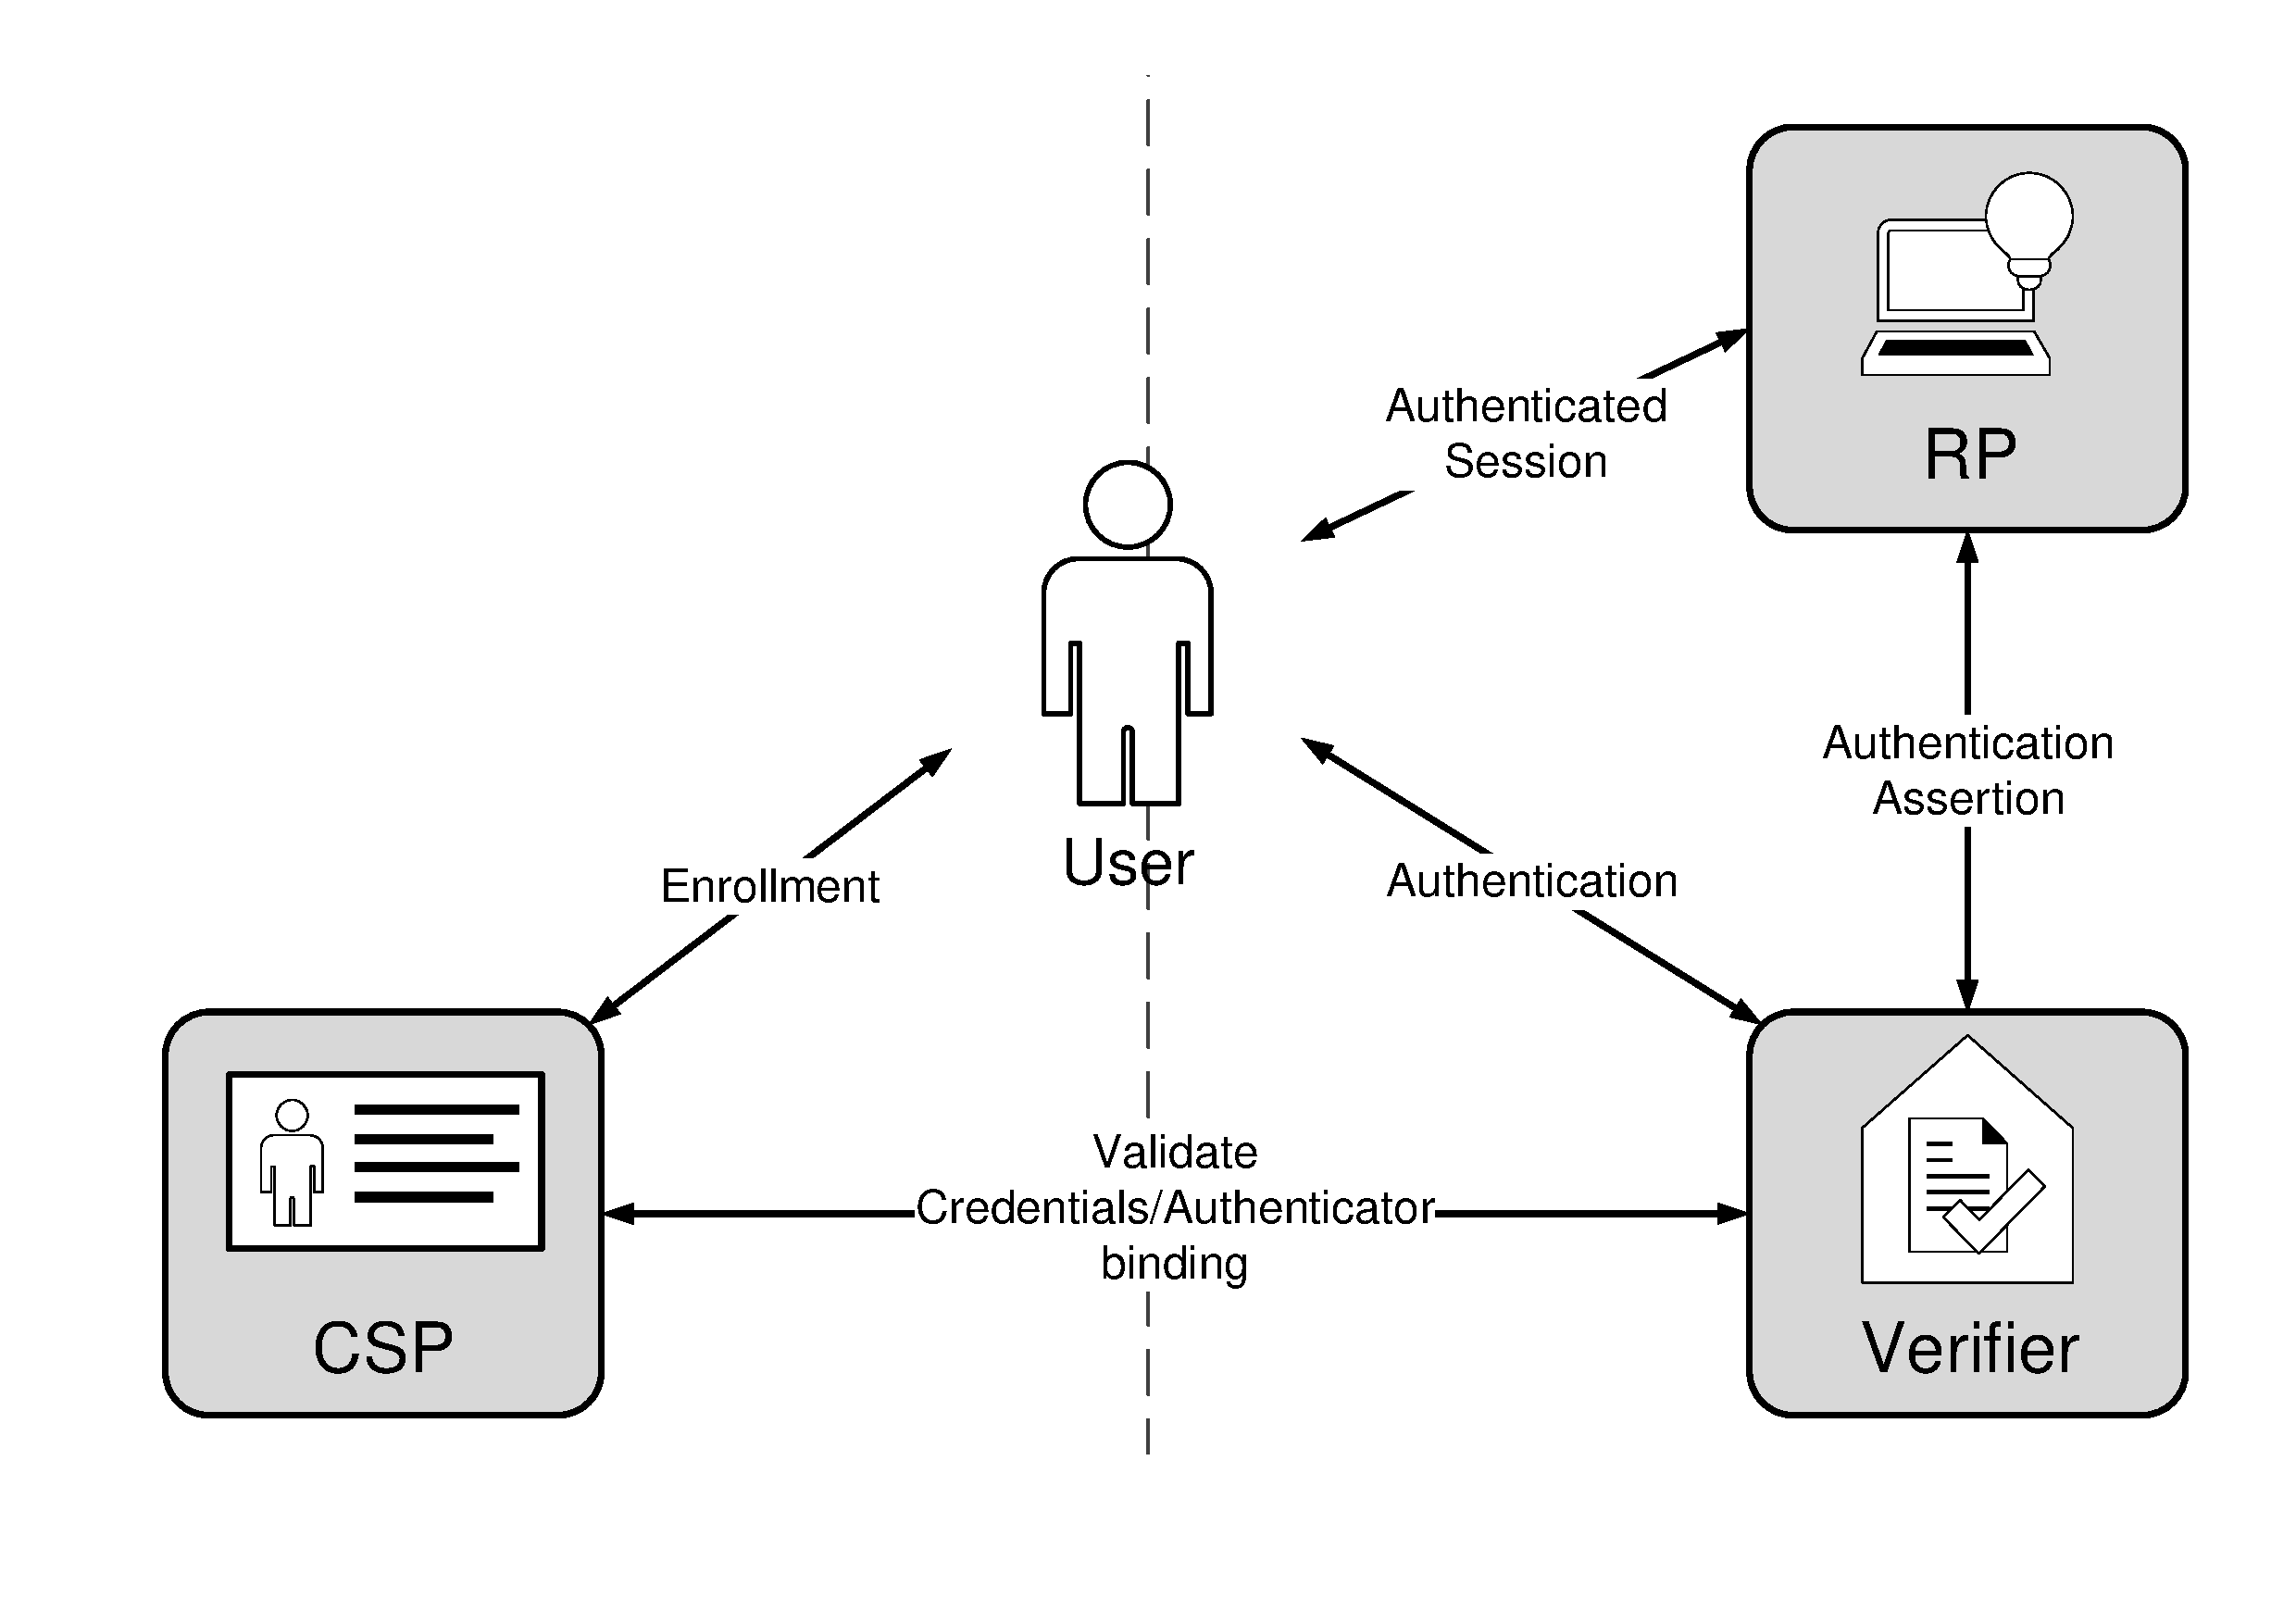
\includegraphics[width=.95\textwidth]{nist-simplified}
    \caption{Digital Identity Model (simplified). The left side of the figure represents enrolment of the user with the \acrshort{csp}. The right part of the user represents authentication with the verifier, before an authenticated session is established between the user and the \acrshort{rp}. Taken from (edited).
    % %REFERENCE Digital identity guidelines: revision 3
    }
    \label{fig:nist-model}
\end{figure}

\paragraph{SP 800-63A}
This volume of the Digital Identity Guidelines defines three Identity Assurance Levels (IALs) and requirements on identity proofing for each level. The \acrshort{ial}1 requires no verification of assertions provided by the user. \acrshort{ial}2 requires either remote or physically-present verification of assertions made by the user, while \acrshort{ial}3 requires manual verification by a trained person, representing the \acrshort{csp}.

% REFERENCE Digital identity guidelines: enrollment and identity proofing

\paragraph{SP 800-63B}
The B volume of the Guidelines defines three Authenticator Assurance Levels (AALs).

To authenticate themselves in AAL1, the user needs to demonstrate control of one authenticator. This must be done through a secure authentication protocol.

In AAL2, the user must demonstrate control of two distinct authenticators. This can be in a form of a multi-factor authenticator, or single-factor possession-based authenticator together with a memorised password. Cryptographic techniques defined in
% REFERENCE SECURITY REQUIREMENTS FOR CRYPTOGRAPHIC MODULES
must be used.

In AAL3, a hardware-based authenticator must be used in addition to requirements of AAL2. Furthermore, one of the authenticators used must be resistant to attacks attempting to impersonate the user.

\paragraph{SP 800-63C}
The C volume of the guidelines describes the use of assertions for identity federation across several \acrshort{rp}s. This enables the user to use services provided by several \acrshort{rp}s, while maintaining only a single identity at one \acrshort{idp}. The volume also describes three Federation Assurance Levels, however we do not cover these in this report.
% REFERENCE Digital identity guidelines: federation and assertions

\paragraph{Authenticator types}

% TODO WRITE HERE

\pagebreak
\section{State of the Art}

In this section we describe the major players on the market of access control solutions. First we focus on online access control, including device log-in, \acrshort{sso} and directory services. Next, we focus on physical and hybrid access control, comprising access control to protected physical premises and hybrid model that offer physical and online access control. For each category we describe a single vendor, who has significant position on the market and who's offering can be used as a benchmark.

\subsection{Online access control -- Microsoft}\label{sec:online-access-control}

For the online access control, we choose Microsoft and its Azure Active Directory (Azure AD)\footnotemark as the benchmark solution, as it is described as ``the leader'' in its field~\cite{Kreizman2018MagicWorldwide}. It offers directory services, user authentication and authorisation of users' application access as the core of its functionality, and is primarily targeted on enterprises and organisations, irrespective of size. Microsoft claims that in 2013 50\% of companies on the Fortune~500 list were already using Azure AD and by 2017, this number has grown to 90\%~\cite{Martin201350Azure}.

\footnotetext{\url{https://azure.microsoft.com/en-us/services/active-directory/}, accessed 25 March 2019}

\paragraph{Authentication} Microsoft Azure AD uses passwords as the primary user authentication method and this setting cannot be changed~\cite{Flores2019AuthenticationMethods}. To provide additional security, \acrlong{mfa} can be enabled. Additional factors that are supported by the solution include:
\begin{enumerate*}[label=(\roman*)]
    % \item \textit{security questions},
    % \item \textit{email address},
    \item \textit{SMS} and \textit{voice call},
    \item \textit{Microsoft Authenticator application},
    \item \textit{one-time passwords}, and 
    \item \textit{OATH hardware tokens}\footnotemark~\cite{Flores2019AuthenticationMethods}.
\end{enumerate*}

Either the enterprise administrator or the user themselves can decide, which of these is used as the second authentication factor. Once enabled, the second factor is always required during user sign-in. Exceptions to this can be defined based on countries, locations, or IP ranges. Moreover, email address and security questions can be added by the user as an additional factor, which can only be used during password recovery, but not during sign-in~\cite{eross-msft2018ConfigureAuthentication}.

\footnotetext{Note, that \acrshort{oath} is different from OAuth. \acrshort{oath} hardware tokens are \acrshort{otp} devices following the reference architecture defined by \acrfull{oath}.

\url{https://openauthentication.org/}, accessed 25 March 2019}

\paragraph{Single Sign-on} Azure AD supports both \acrshort{saml} and OAuth + OpenID Connect for single sign-on to non-Microsoft applications. Developers are encouraged to only use OAuth + OpenID Connect for new applications, but \acrshort{saml} can still be used with legacy and other software that does not support OAuth + OpenID~\cite{barbkess2019SingleDirectory}. 

All four types of authorisation grants defined in OAuth specification can be used. The ID token which is issued during the OpenID connect flow, contains the standard claims defined in the specification. Two endpoints are defined to handle OAuth + OpenID Connect protocols -- v1.0 and v2.0. Together, the two endpoints support variety of languages (.NEt, JavaScript, Python, Java and other) and target applications (on-premise, cloud-based, hybrid)~\cite{deGuzman2018AboutPlatform}.

Azure AD further supports password-based, HTML header-based  and Integrated Windows Authentication \acrlong{sso}~\cite{barbkess2019SingleDirectory}. These are out of scope for this report.

\paragraph{Application access policy management} When a new application is integrated with Azure AD, the access to this application needs to be provisioned to users. This can be done on an individual or a group basis (role-based access control). 

Attribute-based access control is also implemented to a certain degree via use of the \textit{conditional access} method. When this method is in use, additional parameters can be evaluated, such as location, whether \acrshort{mfa} has been used, whether the user is using a compliant device and other predefined attributes. Furthermore, the enterprise administrator can further define custom criteria that need to be met (such as authentication with an external provider)~\cite{Vilcinskas2019WhatAccess}.
\subsection{Physical and hybrid access control -- HID}
\pagebreak
\section{Analysis}\label{sec:analysis}

Building up on our initial idea and problem formulation, we determine two major functional areas that must be supported by our proposed system:

\begin{itemize}[noitemsep]
    \item \textit{\acrfull{pacs}} (access to restricted premises in a company or institution, building access control etc.)
    \item \textit{Online Access Control} (access to computer systems, applications, online sign-in etc.)
\end{itemize}

While the  typical question in a \acrshort{pacs} would be ``\textit{Is the person allowed to enter beyond this point}?'', and can be controlled by a variety of physical barriers, doors, turn-sites and the like, the online access control is more complex. Enterprises nowadays operate a wide spectrum of software solutions including on-premise applications, legacy systems, cloud-based and \acrshort{saas} applications, internally or externally oriented \acrshort{api}s and databases. All of these require some level of access control. To break down this structure, we first begin by identifying two service classes:
\begin{enumerate*}[label=(\roman*)]
    \item \textit{internal applications}, that sit within the enterprise security realm; and 
    \item \textit{external applications}, that include cloud based software, \acrshort{saas} solutions and partner/vendor applications, and which reside outside the given security realm.
\end{enumerate*}

The external applications can be further divided based on their interactions with the internal systems. Applications that are not business critical and/or are not integrated with the business processes may not require access to protected resources at all. Examples of such applications would be a lunch booking system or a company social network. These would be primarily used by the employees, but would not require connectors to business-critical systems and could therefore reside outside the security realm.

Other external applications, however, may require access to business-critical resources for their functions. \acrlong{crm} or payroll system may both be purchased as a \acrshort{saas}, but both require connectors to the protected resources to properly fulfil their functions. We can therefore extend our classification of the external applications accordingly -- applications that
\begin{enumerate*}[label=(\roman*)]
    \item \textit{require access to protected resources} and
    \item \textit{do not require access to protected resources}.
\end{enumerate*}

The access control of \textit{internal applications} will likely differ from access control of \textit{external applications} and similarly, the access control for applications that require access to protected reources will differ from those that do not. We can therefore devise an access control breakdown chart, as shown in Figure~\ref{fig:acs-classification}. 

Multiple sources list Identification, Authentication and Authorisation as the three basic steps in access control~\cite{Harris2008CISSPGuide, 2018AccessSystems, 2003IdentificationAuthorization}. We focus on strong authentication and authorisation in the system design and describe these further in the following sections.

\begin{figure}[ht]
    \centering
    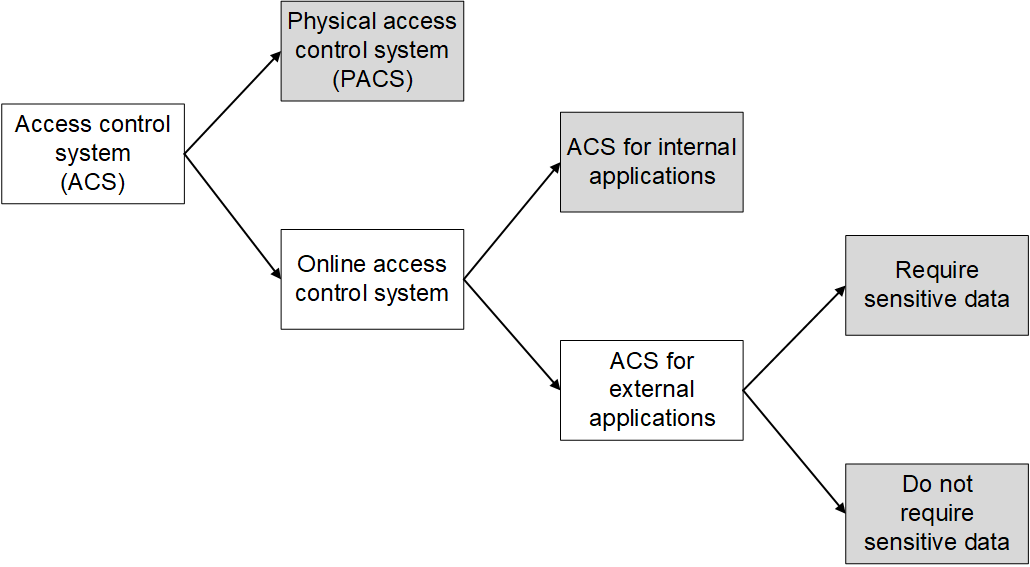
\includegraphics[width=.95\textwidth]{acs-classification}
    \caption{Access control system breakdown chart. \acrshort{acs} for external applications is different for applications work with sensitive data from \acrshort{acs} for external applications that do not work with sensitive data.}
    \label{fig:acs-classification}
\end{figure}

\subsection{Authentication}
In \acrshort{pacs}, physical tokens, such as ID cards, are the common practice nowadays. A survey carried out in 2016 indicated that above 40\% of the companies use low frequency proximity cards as their main method for personal authentication. These cards, operating between 125-134kHz proximity cards are considered an obsolete technology and are not secure~\cite{Hakamaki2015SecurityTechnology}. On the other end of the spectrum, around 20\% of the companies indicated use of mobile devices as a part of their \acrshort{pacs} solution~\cite{HIDGlobal2017TheEnterprise}. 

The main benefit of using a mobile device for this purpose is, that most people already own a smartphone and usually carry it with them at all times. Other technologies represented in the survey that are considered secure today, include iCLASS (contact-less card) and MIFARE DesFire (contact-less card). FIDO, nor FIDO2 keys (NFC, Bluetooth, or other) are not mentioned in the survey, although compatible \acrshort{pacs} systems exist on the market today\footnotemark. 

FIDO and FIDO2 enjoy support of big companies like Google, Facebook and Microsoft, but consumer-oriented application permit the use only as the second authentication factor. Google uses FIDO U2F keys for their employees, but only as a password replacement in the online login scenario~\cite{Krebs2018Google:Phishing} and Microsoft only supports FIDO2 keys with personal Microsoft accounts. As shown in Section~\ref{sec:online-access-control}, even Azure AD does not support this technology. To explore how FIDO2 can be used for hybrid access control on an enterprise scale, we introduce a mandatory support of FIDO2 as a requirement for our system.
% 
\footnotetext{\url{https://web.archive.org/web/20190319221618/https://www.yubico.com/works-with-yubikey/catalog/modis/}, accessed 19 March 2019}

There is already a variate of devices that have been FIDO2 certified, with the Android system being the latest addition to the list~\cite{FIDOAlliance2019AndroidPasswords}. Consideration needs to be put into how the FIDO2 flow will be incorporated in the system and which of the FIDO2-certified devices should be used in the flow. In the \acrshort{pacs}, usability and namely the speed is an important criteria, since existing systems already offer very low- to no-latency during a typical door opening use case. Beyond \acrshort{pacs}, the current access control solutions are above all used for employee identification (as an ID badge)~\cite{HIDGlobal2017TheEnterprise} and the employee is only issued a single badge. The recommended approach in case the employee forgets the badge is to assign a temporary one that can be used during a limited time period and must be returned afterwards~\cite{Ryan2018HowBadges}.

In the online authentication, we can see that the systems support a wider range of authentication (and account recovery) methods, and the user is left to decide, which is authentication method do they prefer. Offering multiple methods simultaneously makes sense for the online access control scenario, because unlike in \acrshort{pacs}, were the on-site reception/security personnel can verify employees identity and issue a temporary badge, in the online access control this is not always possible. In case of forgotten credentials, the identity would therefore needed to be verified remotely (typically over phone), which is not always feasible.

In the proposed hybrid access control system, we must therefore provide an authenticator, that is both fast to use and can be easily complemented and/or substituted with another authentication method if lost or forgotten. We propose the combination of FIDO2 key with \acrshort{nfc} (primary authenticator) and FIDO2 enabled smartphone (supplementary authenticator) to meet the above mentioned criteria. The FIDO2 key with NFC support offers proximity-card-like usability (the user needs to swipe/hold the key next to the reader). If lost or forgotten, it can be substituted by an FIDO2 enabled smartphone, as people generally carry a smartphone with them, while at work.

% TODO FIDO2 would be used for all 4 boxes from access control breakdown chart

% TODO How OpenID connect is used for authentication/SSO
% TODO What information needs to be shared (Default OIDC scope - name, email, UID)...?
% TODO What entities will be needed (OID provider)
% TODO OpenID connect would be used only for boxes 3 and 4 from access control breakdown chart


% For \acrlong{aal}s 2 and 3 defined in 
% %  REFERENCE SECURITY REQUIREMENTS FOR CRYPTOGRAPHIC MODULES
% , authentication must be carried out using at least two independent factors. This requirement, together with abandonment of memorised secrets results in adoption of new authenticators. These  authenticators should offer at better security as memorised secrets, while maintaining the same level of accessibility. In 


% TODO OAuth scopes (SOTA)
% TODO Why we choose OAuth
% TODO Which scopes need to be included
% TODO Which entities will be needed to support this (Authorisation server)

% TODO OAuth will be used for boxes 3 and 4 from access control breakdown chart

\subsection{Access Policy Management}\label{Access_Policy_Management_Analysis}

In every \acrlong{acs}, the model used for granting the access play a crucial role as the system is dependent on it. Often it makes it easier for the administrator to manage and grant the access to employees, but if wrong model is chosen or is wrongly implemented, it can make the work even more burdensome. As it was outlined in the State of the Art (Chapter \ref{SOTA}), we are looking into \acrshort{rbac} and \acrshort{abac} as models for Identity and Access Management as they are the most used ones these days~\cite{2018BestV3}.

Both models offer a range of functionality and suits specific enterprises. One of \acrshort{rbac}’s big advantages is the ease of creating and maintaining the roles and system as a whole, but as the enterprise grows and more roles and resources are introduced, it gets complicated and hard to have an overview. Therefore, \acrshort{rbac} is suitable for small to medium enterprises. It is less complex than \acrshort{abac} and therefore it offers low level of granularity. Permission only can be granted to roles, not to operations or objects. On-the-fly contextual decisions are not supported, as well as restrictions can only be applied to parts of the system, not on specific data. Also, only known parameters can be used during implementation and environmental restrictions cannot be implemented. Even though, \acrshort{rbac} is older model it still offers adequate functionality.

On the other hand, \acrshort{abac} model which is based on attributes and policies presents fine grain and multi-dimensional access control. Biggest advantages of \acrshort{abac} over \acrshort{rbac} are the scalability of the model, dynamic parameters, easy maintenance and support for on-the-fly context aware decisions as information about requesting subject, requested object and environmental attributes are present. This way it is possible to grant access to specific data at specific times based on location. Initial configuration of the system is more complex compared to \acrshort{rbac}, but once done, it is easy to add new attributes or policies which are automatically executed. 

As the focus of the project, is to offer \acrlong{acs} to big enterprises, allowing fine grain control over resources, \acrlong{abac} model is more suitable for the solution. The trend in the industry is to adopt \acrshort{abac} more and more, and Gartner predicts that \textit{``By 2020, 70\% of businesses will use attribute-based access control (\acrshort{abac}) to protect critical assets''}~\cite{GartnerGartnerPredictions}. Studies also shows, that \acrshort{abac} is the model which should be used by enterprises in the future, rather than \acrshort{rbac}~\cite{Fatima2016TowardsArgument}.

To implement \acrshort{abac} model, the standard have to chosen as well. The most wide-spread standard is \acrshort{xacml}, which is explained in Section \ref{sec:xacml}, but others such as \acrfull{alfa} or \acrfull{ngac} exists as well. \acrshort{alfa} is a pseudocode language based on \acrshort{xacml} which provide higher user-friendliness, lower complexity and overall similar performance~\cite{Mejri2016FormalPolicies}. \acrshort{ngac} on the other hand, even-though it uses \acrshort{abac} model for access control, its implementation differs from \acrshort{xacml}~\cite{Ferraiolo2016ANGAC}. For the purpose of this project, we decide and propose the use of \acrshort{xacml} as the standard for implementing \acrshort{abac} in the system, mainly because of its wide spread, similar functionality to \acrshort{ngac} and the fact that it is being taught at the Identity and Access Management course at the university.
\pagebreak
\section{Design}

% TODO section intro

% TODO decide order of the sections
\subsection{Architecture}
In this section we explain the entities of the proposed system and their roles. Afterwards, we present high-level sequence diagrams of the system for the basic use cases. We explain what messages flow among the system components and how these represent the individual authentication and authorisation flows explained in the \href{sec:analysis}{Analysis section}.

\subsubsection{System Components}
To best design the architecture of our system, we must first understand the different actors and their roles. Investigating the specifications of FIDO2, OAuth and \acrshort{oidc} might give us an idea of what the necessary components might be, but there is a degree in ambiguity in these specifications -- the problem being, that while each specification does a good job explaining details in its own context, in order to bring an access control system to life, we must understand where these contexts intersect each other.

In FIDO2, the typical parties are \textit{authenticator}, \textit{client} and \textit{\acrshort{rp}}. In OAuth, we have the following entities: \textit{user agent}, \textit{client application} and \textit{authorisation server}. In \acrshort{oidc} we have \textit{relying party}, \textit{OIDC provider}, \textit{token endpoint} and so on. To avoid this naming overlap, we identify the following entities as our system components:
% 
\begin{itemize}
    \item \textit{Client application} is the business application the user is about to use. If this is an internal application, it would typically have direct access to protected resources. If this is an external application, it would typically require an OAuth access token to access the protected resources.
    
    Client application can be either of the three client types that are recognised by the OAuth specification~\cite{Hardt2012TheFramework} -- web based application (running on a web server), user-agent-based application (downloaded from the web server, but executed locally) or a native application.
    
    Examples of client application are: Slack, Salesforce, ServiceNow or Zendesk.
    
    \item \textit{User agent} interacts with the user during the login and authentication. It displays forms for username input and communicates with the physical authenticator device via CTAP2 protocol. This is typically a web browser. I should be able display HTML and handle the CTAP2 flow with the host OS. Principally, it could be both desktop- and mobile-based (currently only on the Android mobile platform). In FIDO2, this would be named as client or client device.
    
    Examples are: Chrome, Mozilla, Microsoft Edge.
    
    \item \textit{Authorisation Server}
    
    \item \textit{User attribute database (or User DB)}
    
    \item \textit{Policy Enforcement Point (PEP)}
    
    \item \textit{API endpoint}
\end{itemize}
% 
\pagebreak

\printbibliography[heading=bibintoc]

% \epigraph{Smart contracts are neither smart, nor contracts!}{\textit{www.stateofthedapps.com/about}}

\pagebreak

\appendix
% \newgeometry{left=1cm,right=1cm,top=1cm,bottom=1cm,footskip=.4cm}
\section{SAML and OAuth + OpenID Connect support in enterprise applications}\label{sec:appendix-links}

\paragraph{Zendesk} Only supports SAML:

\url{https://support.zendesk.com/hc/en-us/articles/203663676}, accessed on 31 March 2019 (\href{https://web.archive.org/web/20190331182733/https://support.zendesk.com/hc/en-us/articles/203663676}{view archive version}).

\url{https://support.zendesk.com/hc/en-us/community/posts/115006523287-Does-Zendesk-Support-OpenID-Connect-}, accessed on 31 March 2019 (\href{https://web.archive.org/web/20190331182849/https://support.zendesk.com/hc/en-us/community/posts/115006523287-Does-Zendesk-Support-OpenID-Connect-}{view archive version}).

\paragraph{Slack} Only supports SAML:

\url{https://get.slack.help/hc/en-us/articles/203772216-SAML-single-sign-on}, accessed on 31 March 2019 (\href{https://web.archive.org/web/20190331183030/https://get.slack.help/hc/en-us/articles/203772216-SAML-single-sign-on}{view archive version}).

\paragraph{Salesforce} Supports both SAML and OAuth + OpenID Connect:

\url{https://help.salesforce.com/articleView?id=sso_saml.htm&type=5}, accessed on 31 March 2019 (\href{https://web.archive.org/web/20190331183852/https://help.salesforce.com/articleView?id=sso_saml.htm&type=5}{view archive version}).

\url{https://help.salesforce.com/articleView?id=sso_provider_openid_connect.htm&type=5}, accessed on 31 March 2019 (\href{https://web.archive.org/web/20190331184051/https://help.salesforce.com/articleView?id=sso_provider_openid_connect.htm&type=5}{view archive version}).

\paragraph{ServiceNow} Supports both SAML and OAuth + OpenID Connect:

\url{https://docs.servicenow.com/bundle/london-platform-administration/page/administer/security/task/add-OIDC-entity.html}, accessed on 31 March 2019 (\href{https://web.archive.org/web/20190331184433/https://docs.servicenow.com/bundle/london-platform-administration/page/administer/security/task/add-OIDC-entity.html}{view archive version}).

\url{https://docs.servicenow.com/bundle/london-platform-administration/page/integrate/saml/concept/c_SAML2.0WebBrowserSSOProfile.html}, accessed on 31 March 2019 (\href{https://web.archive.org/web/20190331184648/https://docs.servicenow.com/bundle/london-platform-administration/page/integrate/saml/concept/c_SAML2.0WebBrowserSSOProfile.html}{view archive version}).
% \newgeometry{left=1cm,right=1cm,top=1cm,bottom=1cm,footskip=.4cm}
% \section{Smart contract code}\label{sec:appendix-code}
\begin{figure}[H]
    \centering
    \includegraphics[height=0.90\textheight]{code-smart-contract}
    \label{fig:smart-contract-code}
\end{figure}
\restoregeometry
% \newgeometry{left=2cm,right=2cm,top=1cm,bottom=1cm,footskip=.4cm}
% \section{Implemented requirements table}\label{sec:appendix-table}
\begin{table}[H]
    \centering
    \begin{tabularx}{\textwidth}{|l X c|}
    \hline
    \textbf{ID}&\textbf{Description}&\textbf{Implemented}\\
    % 
    \multicolumn{3}{|c|}{\textbf{Application front end}}\\
    AF-FR-1&Application must deploy the smart contract to an Ethereum node.&Yes\\
    AF-FR-2&Application must be able to query the node for address balance.&Yes\\
    AF-FR-3&Application must display the status of the transaction.&Yes\\
    AF-NFR-1&Transaction must be signed on device.&Yes\\
    AF-NFR-2&Sensitive details about users' funds must not leave the device.&Yes\\
    % 
    \multicolumn{3}{|c|}{\textbf{Ethereum node}}\\
    EN-FR-1&Node must support at least the following methods of the JSON-RPC protocol: \texttt{eth\_getBalance} and \texttt{eth\_sendTransaction}.&Yes\\
    EN-NFR-1&Node should process method calls without delay.&\textbf{No}\\
    EN-NFR-2&Node should process all method calls with equal priority.&\textbf{No}\\
    EN-NFR-3&Node should inform the application about the outcome of the method call.&\textbf{No}\\
    % 
    \multicolumn{3}{|c|}{\textbf{Smart contract}}\\
    SC-FR-1&The smart contract must implement the logic described in~\ref{fig:simple-logic}.&Yes\\
    SC-NFR-1&The smart contract must emit en event after contract creation.&Yes\\
    SC-NFR-2&The smart contract must cover the costs for the services of the oracle.&\textbf{No}\\
    SC-NFR-3&The smart contract could emit an event upon receiving a response from the oracle.&Yes\\
    % 
    \multicolumn{3}{|c|}{\textbf{Oracle}}\\
    OR-FR-1&The oracle must support queries to a web \acrshort{api}.&Yes\\
    OR-NFR-1&The oracle should provide accurate and correct response to the query.&\textbf{No}\\
    OR-NFR-2&The oracle should respond to queries without delay (unless otherwise specified).&\textbf{No}\\
    %   
    \multicolumn{3}{|c|}{\textbf{Blockchain explorer}}\\
    BE-FR-1&Blockchain explorer must support an API query for address balance.&Yes\\
    BE-NFR-1&The blockchain explorer should provide accurate and correct response to the query.&\textbf{No}\\
    BE-NFR-2&The blockchain explorer should respond to queries without delay.&\textbf{No}\\
    % 
    \multicolumn{3}{|c|}{\textbf{Communication back end}}\\
    CB-FR-1&Communication back end should be able to store users' offers.&Yes\\
    CB-FR-1&Communication back end should assist users during the transaction process.&Yes\\
    CB-NFR-1&The communication back end must not be able to prevent a transaction from happening.&\textbf{No}\\
    CB-NFR-2&The communication back end must not have control over users' funds.&Yes\\
    \hline
    \end{tabularx}
    % \caption{//write}
    \label{tab:component-reqs-eval}
\end{table}

% \newgeometry{left=1cm,right=1cm,top=1cm,bottom=1cm,footskip=.4cm}
% \section{Transaction process screenshots}\label{sec:appendix-screenshots}

% //ADD Screensoht descriptions

    \centerline{\includegraphics[width=0.75\textwidth]{screenshots/screen020}}
    \centerline{\includegraphics[width=0.75\textwidth]{screenshots/screen031}}
    \textit{Top:}    Front page of the application\\
    \textit{Bottom:} The secondary user clicked on \textit{Create new offer}.\\
    \centerline{\includegraphics[width=0.85\textwidth]{screenshots/screen032}}
    \centerline{\includegraphics[width=0.85\textwidth]{screenshots/screen033}}
    \textit{Top:}    The secondary user filled in the details of the Bitcoin offer.\\
    \textit{Bottom:} The secondary user clicked on \textit{OR} button to scan the destination Ethereum address.\\
    \centerline{\includegraphics[width=0.85\textwidth]{screenshots/screen034}}
    \centerline{\includegraphics[width=0.85\textwidth]{screenshots/screen041}}
    \textit{Top:}    The Ethereum address was filled by the QR code scan.\\
    \textit{Bottom:} The secondary user clicked on \textit{Create new offer}.\\
    \centerline{\includegraphics[width=0.85\textwidth]{screenshots/screen042}}
    \centerline{\includegraphics[width=0.85\textwidth]{screenshots/screen043}}
    \textit{Top:}    The primary user selected the offer from the list.\\
    \textit{Bottom:} The primary user clicked on \textit{Continue}. A screen prompting them to transfer funds to said Ethereum address was displayed.\\
    \centerline{\includegraphics[width=0.85\textwidth]{screenshots/screen051}}
    The primary user clicked on \textit{Continue}. A screen prompting them to fill in their Bitcoin address was displayed. The Ethereum address and Bitcoin address are pre-filled.\\
    \centerline{\includegraphics[width=0.85\textwidth]{screenshots/screen060}}
    The primary user deposited Ether to the temporary Ethereum address.\\
    \centerline{\includegraphics[width=0.85\textwidth]{screenshots/screen071}}
    \centerline{\includegraphics[width=0.85\textwidth]{screenshots/screen072}}
    \textit{Top:}    The balance of the temporary Ether wallet has changed.\\
    \textit{Bottom:} The primary user filled in their Bitcoin address.\\
    \centerline{\includegraphics[width=0.80\textwidth]{screenshots/screen081}}
    \centerline{\includegraphics[width=0.80\textwidth]{screenshots/screen082}}
    \textit{Top:}    The primary user clicked on \textit{Validate}. This displayed a validation screen and triggered a prompt at the secondary user's device.\\
    \textit{Bottom:} Secondary user pressed \textit{Yes}. This action changed the colour of the \textit{Yes} button on primary user's screen.\\
    \centerline{\includegraphics[width=0.80\textwidth]{screenshots/screen091}}
    \centerline{\includegraphics[width=0.80\textwidth]{screenshots/screen092}}
    \textit{Top:}    A transaction hash was displayed to the primary user and a link to blockchain explorer was displayed to both users.\\
    \textit{Bottom:} The secondary user clicked on \textit{Continue}. This displayed a screen, prompting them to transfer the Bitcoin\\    
    \centerline{\includegraphics[width=0.85\textwidth]{screenshots/screen100}}
    The secondary user transferred the Bitcoin to the primary user.\\
    \centerline{\includegraphics[width=0.85\textwidth]{screenshots/screen110}}
    Response from Oraclize.
    

% \restoregeometry

\end{document}